\documentclass[12pt]{amsart}

%auto-ignore
%this ensures the arxiv doesn't try to start TeXing here.
%!TEX root=exceptional.tex
\usepackage{amssymb}
\usepackage{array}
\usepackage{booktabs}
\usepackage{mdwtab}
\usepackage{mathtools}
\usepackage[T1]{fontenc}
\usepackage[utf8]{inputenc}
\usepackage{libertine}
\usepackage[libertine]{newtxmath}
\usepackage{hyphenat}
\usepackage{enumitem}
\usepackage{xcolor}
\definecolor{medium-blue}{rgb}{0,0,0.65}
\usepackage{ifpdf}
\ifpdf
  \usepackage[pdftex]{graphicx}
  \usepackage[pdftex,margin=1.25in]{geometry}
  \usepackage[bookmarks=true, bookmarksopen=true,%
    bookmarksdepth=3,bookmarksopenlevel=2,%
    colorlinks=true,%
    linkcolor=purple,%
    citecolor=medium-blue,%
    filecolor=blue,%
    menucolor=blue,%
    urlcolor=medium-blue]{hyperref}
  \hypersetup{pdftitle={Towards the quantum exceptional series}}
  \hypersetup{pdfauthor={Scott Morrison, Noah Snyder, and Dylan P. Thurston}}
\else
  \usepackage[dvips]{graphicx}
  \usepackage[dvips,margin=1in]{geometry}
  % Use hyperref with all features turned off even in DVI mode, since
  % the .aux file format changes
  \usepackage[draft]{hyperref}
\fi
\usepackage{url}
\usepackage{todonotes}
\usepackage{tikz}
\usetikzlibrary{shapes}
\usetikzlibrary{calc}
\usetikzlibrary{knots}

\usepackage[backend=biber,style=alphabetic,doi=false,isbn=false,url=false,minnames=6,maxnames=6]{biblatex}
\setcounter{biburlnumpenalty}{9000}
\setcounter{biburllcpenalty}{1000}
\setcounter{biburlucpenalty}{8000}
\renewbibmacro{in:}{%
  \ifentrytype{article}{}{\printtext{\bibstring{in}\intitlepunct}}}
\renewbibmacro*{volume+number+eid}{%
  \printtext{vol.}
  \printfield{volume}%
  \setunit*{\addnbspace}% NEW (optional); there's also \addnbthinspace
  \printfield{number}%
  \setunit{\addcomma\space}%
  \printfield{eid}}
\DeclareFieldFormat[article]{number}{\mkbibparens{#1}}
\usepackage{silence}
% Filter warnings issued by package biblatex starting with "Patching footnotes failed"
\WarningFilter{biblatex}{Patching footnotes failed}
\addbibresource{bibliography/bibliography.bib}

% A binary operator with a subscript on both sides (and correct spacing)
% Name stands for subscript-operator-subscript
\newcommand{\sos}[3]{\mathbin{{}_{#1}\mathord#2_{#3}}}

% manyindices
% Adapted from code by "bza" in comp.text.tex, Feb. 7, 2006
%% USAGE:
%%
%% \manyindices#1#2#3#4#5
%%
%% #1=lower left index
%% #2=upper left index
%% #3=lower right index
%% #4=upper right index
%% #5=main symbol
\makeatletter
\newcommand\mi@kern[1]{%
  \settowidth\@tempdima{$\mi@obj^{#1}$}
  \kern-\@tempdima
  #1
  \settowidth\@tempdima{$\mi@obj$}
  \kern\@tempdima
}

\newtoks\mi@toksp
\newtoks\mi@toksb
\DeclareRobustCommand{\manyindices}[5]{
  \def\mi@obj{#5}
  \mi@toksp\expandafter{\mi@kern{#2}}
  \mi@toksb\expandafter{\mi@kern{#1}}
  \@mathmeasure4\textstyle{#5_{#1}^{#2}}
  \@mathmeasure6\textstyle{#5_{#3}^{#4}}
  \dimen0-\wd6 \advance\dimen0\wd4
  \@mathmeasure8\textstyle{\hphantom{{}_{#1}^{#2}}#5^{\the\mi@toksp#4}_{\the\mi@toksb#3}}
  \hbox to \dimen0{}{\kern-\dimen0\box8}
}
\makeatother 

% Left sub/super scripts
% \lsup is a temporary definition until something better is worked out
% Use \lsupv if the next argument is vertical
\newcommand{\lsub}[2]{{}_{#1}#2}
\newcommand{\lsup}[2]{{}^{#1}\mskip-.6\thinmuskip#2}
\newcommand{\lsupv}[2]{{}^{#1}#2}
\newcommand{\lsubsup}[3]{\manyindices{#1}{\mskip.6\thinmuskip#2\mskip-.6\thinmuskip}{}{}{\mathord{#3}}}
\newcommand{\lsubsupv}[3]{\manyindices{#1}{\mskip.2\thinmuskip#2\mskip-.2\thinmuskip}{}{}{\mathord{#3}}}

\newcounter{saveenum}

% Read the file, if it exists
\newread\testin
\def\maybeinput#1{
\openin\testin=#1
\ifeof\testin\typeout{Warning: input #1 not found}\else\input#1\fi
\closein\testin
}

\def\mathcenter#1{%
  \vcenter{\hbox{$#1$}}%
}

\def\graph#1{
        \includegraphics{#1}
}

\def\mathgraph#1{
        \mathcenter{\graph{#1}}
}

\def\mfig#1{
        \mathcenter{\includegraphics{#1}}
}

\def\mfigb#1{
        \mathcenter{\includegraphics[trim=-1 -1 -1 -1]{#1}}
}


%%% Local Variables: 
%%% mode: latex
%%% TeX-master: "main"
%%% End: 

% General use
\newcommand{\RR}{\mathbb R}
\newcommand{\CC}{\mathbb C}
\newcommand{\ZZ}{\mathbb Z}
\newcommand{\QQ}{\mathbb Q}
\newcommand{\PP}{\mathbb P}
\newcommand{\EE}{\mathbb E}
\newcommand{\HH}{\mathbb H}
\newcommand{\NN}{\mathbb N}

\newcommand{\comma}{\mathbin ,}
\newcommand{\conn}{\mathbin \#}
\newcommand{\sltwo}{{{\mathfrak{sl}}_2}}
\renewcommand{\sl}{\mathfrak{sl}}
\newcommand{\gl}{\mathfrak{gl}}
\newcommand{\fg}{{\mathfrak g}}
\newcommand{\co}{\colon\thinspace}
\newcommand{\eps}{\varepsilon}
\newcommand{\abs}[1]{{\lvert #1 \rvert}}
\newcommand{\norm}[1]{{\lVert #1 \rVert}}
\newcommand{\OneHalf}{{\textstyle\frac{1}{2}}}

% Synonyms for commands I never remember
\newcommand{\isom}{\cong}
\newcommand{\superset}{\supset}
\newcommand{\bigcircle}{\bigcirc}
\newcommand{\contains}{\ni}
\newcommand{\tensor}{\otimes}
\newcommand{\bdy}{\partial}

% Stupid overloading.
\newcommand{\lbracket}{[}
\newcommand{\rbracket}{]}

% Various operators.
\DeclareMathOperator{\ad}{ad}
\DeclareMathOperator{\Ad}{Ad}
\DeclareMathOperator{\End}{End}
\DeclareMathOperator{\sign}{sign}
\DeclareMathOperator{\Sym}{Sym}
\DeclareMathOperator{\tr}{tr}
\DeclareMathOperator{\Hom}{Hom}
\DeclareMathOperator{\vol}{vol}
\DeclareMathOperator{\rank}{rank}
\DeclareMathOperator{\im}{im}

% Linear groups
\DeclareMathOperator{\ISO}{\mathit{ISO}}
\DeclareMathOperator{\SO}{\mathit{SO}}
\DeclareMathOperator{\GL}{\mathit{GL}}
\DeclareMathOperator{\SL}{\mathit{SL}}
\DeclareMathOperator{\PSL}{\mathit{PSL}}

% citations
\newcommand{\arxiv}[1]{\href{http://arxiv.org/abs/#1}{\tt arXiv:\nolinkurl{#1}}}
\newcommand{\doi}[1]{\href{http://dx.doi.org/#1}{{\tt DOI:#1}}}
\newcommand{\euclid}[1]{\href{http://projecteuclid.org/getRecord?id=#1}{{\tt #1}}}
\newcommand{\mathscinet}[1]{\href{http://www.ams.org/mathscinet-getitem?mr=#1}{\tt #1}}
\newcommand{\googlebooks}[1]{(preview at \href{http://books.google.com/books?id=#1}{google books})}
\renewcommand{\googlebooks}[1]{}
\newcommand{\numdam}[1]{\href{http://www.numdam.org/item?id=#1}{\tt #1}}

% Theorems
\theoremstyle{plain}
\newtheorem{theorem}{Theorem}
\newtheorem{proposition}{Proposition}
\numberwithin{proposition}{section}
\newtheorem{lemma}[proposition]{Lemma}
\newtheorem{corollary}[proposition]{Corollary}
\newtheorem{claim}[proposition]{Claim}
\newtheorem{conjecture}[proposition]{Conjecture}
\newtheorem{observation}[proposition]{Observation}

\theoremstyle{definition}
\newtheorem{definition}[proposition]{Definition}
\newtheorem{exercise}[proposition]{Exercise}
\newtheorem{question}[proposition]{Question}
\newtheorem{problem}[proposition]{Problem}

\theoremstyle{remark}
\newtheorem{example}[proposition]{Example}
%\newtheorem{hint}[proposition]{Hint}
\newtheorem{remark}[proposition]{Remark}
%\newtheorem{apology}[proposition]{Apology}
%\newtheorem{warning}[proposition]{Warning}

% Hyphenation.
\hyphenation{Thurs-ton}

%ToDoNotes:
\newcommand{\nn}[1]{{\color{red}[[#1]]}}
\newcommand{\DPTtodo}[1]{\todo[color=green!40]{#1}}
\newcommand{\NStodo}[1]{\todo[color=blue!40]{#1}}
\newcommand{\SMtodo}[1]{\todo[color=red!40]{#1}}
\newcommand{\citationneeded}{\ \parbox{1.25in}{\todo[inline]{citation needed}}\ }
\newcommand{\referenceneeded}{\ \parbox{1.35in}{\todo[inline]{reference needed}}\ }

% Commands for exceptional paper
\newcommand{\Sk}[1]{\mathop{\mathrm{Sk}}(#1)}
\newcommand{\Skq}[1]{\mathop{\mathrm{Sk}_q}(#1)}
\newcommand{\Skcat}{\mathop{\mathsf{Sk}}}
\newcommand{\Skqcat}{\mathop{\mathsf{Sk}_q}}
\DeclareMathOperator{\eval}{eval}

\DeclareMathOperator{\Tw}{Tw}
\DeclareMathOperator{\HTw}{HTw}
\DeclareMathOperator{\Fr}{Fr}

\DeclareMathOperator{\fork}{fork}
\DeclareMathOperator{\fuse}{fuse}


%%% Local Variables: 
%%% mode: latex
%%% TeX-master: "main"
%%% TeX-master: t
%%% End: 


\begin{document}
\title{Link invariants from the quantum exceptional series}

\author[Morrison]{Scott Morrison}
\address{Mathematical Sciences Institute, Australian National University}
\email{scott.morrison@anu.edu.au}

\author[Snyder]{Noah Snyder}
\address{Bloomington, Indiana, USA}
\email{nsnyder1@indiana.edu} % Noah, do you prefer a different e-mail address?

\author[Thurston]{Dylan~P.~Thurston}
\address{Bloomington, Indiana, USA}
\email{dpthurst@indiana.edu}

\maketitle

\newcommand{\V}{\mathcal{P}}


\section{Link invariants}
\subsection{Matrices}
Recall that we have candidate bases for $\V_n = \operatorname{Hom}(1 \to V^{\otimes n})$, for $n$ at most 6.
In this section, we obtain matrices for the braiding and rotation operators on $\V_n$.

We have a pairing $\langle - , - \rangle: \V_n \otimes \V \to \V_0$ defined by 
\[
  \langle x, y \rangle =
  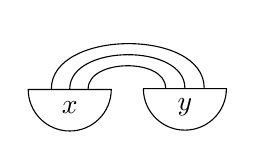
\begin{tikzpicture}[baseline]
    \node[draw, shape=semicircle, shape border rotate=180, minimum size=1.5em] (x) {$x$};
    \node[draw, shape=semicircle, shape border rotate=180, minimum size=1.5em, right=0.5cm of x] (y) {$y$};
    \draw (x.90) to[in=90, out=90] (y.90);
    \draw (x.135) to[in=90, out=90] (y.45);
    \draw (x.45) to[in=90, out=90] (y.135);
  \end{tikzpicture}
\]
and for many 
(conjecturally all) diagrams in $\V_0$ we can use the relations to evaluate to a rational function 
in \(\QQ(v,w)\). Of course, our basis is far from orthonormal with respect to this pairing!
We find, however, that up to $n=6$, we can evaluate all matrix entries of
$M_n = \left(\langle e_i, e_j \rangle\right)_{i,j}$,
but rather unfortunately inverting this matrix is computationally infeasible for $n=6$.
(Recall that arithmetic over $\QQ(v,w)$ is quite inefficient!)

Now, given an operator $T: \V_n \to \V_m$, the associated matrix with respect to our chosen basis is
$AM_m^{-1}$, where $A = \left(\langle T e_i, e_j \rangle\right)_{i,j}$. We find that for
$T$ any of 
\begin{align*}
  (\rho_n : \V_n \to \V_n) & = 
    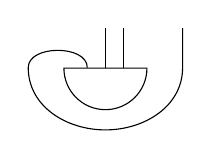
\begin{tikzpicture}[baseline]
      \node[draw, shape=semicircle, shape border rotate=180, minimum size=1.5em] (x) {};
      \draw (x.90) -- ++(0,0.5);
      \draw (x.45) -- ++(0,0.5);
      \draw (x.135) to[in=90, out=90] ++(-0.75,0) 
                     to[in=180,out=-90] ($(x.-90)+(0,-0.25)$) 
                     to[out=0,in=-90] ($(x.45)+(0.75,0)$)
                     -- ++(0,0.5);
    \end{tikzpicture} \\
  (\beta_n : \V_n \to \V_n) & = 
  \\
  (\cap_n : \V_n \to \V_{n-2}) & = 
  \\
  (\cup_n : \V_n \to \V_{n+2}) & = 
  \\
  (\fork_n : \V_n \to \V_{n+1}) & = 
  \\
  (\fuse_n : \V_n \to \V_{n-1}) & = 
  \\
  (H_n : \V_n \to \V_n) & = 
\end{align*}
for values of $n$ so that source and target are amongst $\V_0, \ldots, \V_6$,
we can evaluate all of the matrix entries of $A$ as rational functions.
(Even though $H_n = \rho_{n}^{-1} \fuse_n \rho_{n+1} \fork_n$, 
this does not allow us to compute the matrix for $H_6$, so we need to find this directly.)

Even though directly inverting $M$ is infeasible, we find that we can
calculate the product $A M^{-1}$ in each case.
(Nevertheless this remains a difficult calculation. \nn{some explanation of what we do, with the CRT})

Explicit matrices are available with the {\tt arXiv} sources of this article, as the files {\tt /matrices/OP-n.m}, where {\tt OP} is one of {\tt rotation}, {\tt braiding}, {\tt cup}, {\tt cap}, {\tt fork}, {\tt fuse}, {\tt H}. The matrices are written in terms of the variables $d, v$. \SMtodo{actually create these files}

\subsection{Limited planar operations}
Thinking of the vector spaces $\V_n$ as forming a planar algebra, 
at this point we have limited access to the full set of operations indexed by planar tangle. We have computed above
$\cap_n : \V_n \to \V_{n-2}$, 
$\cup_n : \V_n \to V_{n+2}$, and
$\rho_n: \V_n \to \V_n$. We can also find
\begin{align*}
(m_{4,4,2} : \V_4 \otimes \V_4 \to \V_4) & = ... \\
(m_{4,6,2} : \V_4 \otimes \V_6 \to \V_6) & = ... \\
\intertext{and}
(m_{4,4,1} : \V_4 \otimes \V_4 \to \V_6) & = ... 
\end{align*}
 as follows.

Recall that our chosen basis for $\V_4$ is
\[
  \left(
    ...
  \right)
\]
Expressed in our chosen bases, we then have 
\begin{align*}
  m_{4,n,2}((x_1, x_2, x_3, x_4, x_5) \otimes y)
    & = x_1 \cup_{n-2}\cap_n y \\
      & \quad + x_2 y \\
      & \quad + x_3 \fork_{n-1}\fuse_n y \\
      & \quad + x_4 H_n y \\
      & \quad + x_5 \beta y.
\end{align*}
Finally, we can write $m_{4,4,1}$ in terms of the other operations, as \nn{...}


\subsection{Links with Conway width 6}
Typically, we may choose to think about a diagrammatically defined tangle invariant as a 
morphism of planar algebras $\operatorname{Tangle} \to \mathcal{Q}$ for some planar algebra 
$\mathcal{Q}$,
sending the crossing to a suitable element of $\mathcal{Q}_4$. In our case we only know a 
limited set of operations in the target planar algebra, and so can only compute the invariants
of links which we can generate from the crossing using those available planar operations.

\begin{definition}
The \emph{width} of a planar graph generically embedded in the plane is the maximum number of intersections with a
horizontal line. The width of a planar graph is the minimum width over all generic embeddings.

The \emph{Conway width} of a 4-valent planar graph is the width of the graph after repeatedly collapsing all digons.
The Conway width of a link is the Conway width of its shadow.
\end{definition}

It is easy to see that with the available planar operations, we can evaluate all Conway width 6 links.

\begin{lemma}
All knots and links with at most 12 crossings except 
the alternating link with shadow the cuboctahedron 
have Conway width at most 6.
\end{lemma}
\begin{proof}
\nn{... Conway}
\end{proof}
In fact, almost all prime knots up to 11 crossings have width at most 6, 
with 15 exceptions, all Montesinos knots. Montesinos knots
are easily seen to have Conway width 4.%
\footnote{The exceptions are 11a43, 11a44, 11a47, 11a57, 11a231,
  11a263, 11n71, 11n72, 11n73, 11n74, 11n75, 11n76, 11n77, 11n78, and
  11n81.}

The obvious greedy algorithm (repeatedly collapse digons, when that is not possible apply 
$m_{4,4,1}$ to merge two 4-boxes into a 6-box, and afterwards hope that $m_{6,4,2}$ 
suffices to combine all remaining 4-boxes into that 6-box) works on all but one prime knot up to
12 crossings, except \nn{... is it worth explaining this? perhaps it illustrates the greedy algorithm}

\subsection{Knotted trivalent graphs}
\nn{just some examples}
\nn{including the unknotted dodecahedron}

\subsection{A 2-variable polynomial invariant}
Using the above observations, we have computed the (conjectural!) invariant $\xi$ of all
prime links up to 11 crossings, and all prime knots up to 12 crossings. We observe that the values
of $\xi$ are always of the form
$$\xi(L) - d^{k} = 
\frac{[3][4][\lambda-6][\lambda+5]}{[1][2][\lambda-1]^{k+1} [\lambda]^{k+1}} \mathcal E(L),$$
where $d = \xi(\textrm{unknot}) = ...$, $k$ is the number of components of $L$, 
and $\mathcal E(L)$ is some Laurent polynomial
(not just a rational function) in $v$ and $w$.
These polynomials $\mathcal E (L)$ are tabulated
\nn{ at ...}, and in machine readable format as \nn{...} in the {\tt arXiv} sources.

It would be desirable to verify that these computed invariants specialize correctly to the
quantum link invariants of the adjoint representations of the exceptional Lie algebras.
Unfortunately, these invariants have previously been rather hard to compute, so there is little
available to check against. The Lie algebra $\mathfrak{sl}_2$ lies on the exceptional curve, and
so the 2nd coloured Jones polynomial 
(that is, colored by the 3-dimensional adjoint representation) 
should be the \nn{$w = ...,  v= ...$} specialisation. This is indeed the case for all the links
tabulated above.

Even for the adjoint representation of $G_2$, an earlier program by the first author
for computing quantum knot invariants gets only as far as the trefoil. Sure enough, we have
$$\xi(3_1) = ...$$
which at \nn{$w = ...,  v= ...$} gives \nn{...}

The fact that $\xi(12^n_{...}) = ...$ suggests that the $E_8$ adjoint quantum knot invariant should be
$$...$$, but previous methods haven't come close to computing this.


\end{document}
